\chapter{Présentation}

\section{Auteur}

\noindent
Corentin POUPRY, étudiant à l'ESIEE Paris en E1, promotion 2025.

\section{Thème}

\noindent
Murphy Law, un détective, doit faire la lumière sur l'enquête confiée.

\section{Résumé du scénario}

Vous vous attendiez à tomber sur un super jeu de science-fiction proposé par un étudiant talentueux. Cependant, la réalité est tout autre et vous vous retrouvez au bureau d'un curieux détective. Ce détective, bien décidé à vous aider à faire la lumière sur votre cas atypique, c'est Murphy Law, et c'est lui qu'on appelle quand tout va mal.

\section{Scénario détaillé}

Le Joueur (notons la majuscule) est un personnage à part entière de l'histoire, bien que l'utilisateur joue au travers de Murphy Law. Le Joueur apparaît au début de la narration complètement perdu et à la recherche du jeu de science-fiction promis par le talentueux étudiant dans son rapport. Murphy Law, détective, se demande par quel moyen Le Joueur a pu arriver dans son agence alors que, manifestement, il ne fait même pas partie du schéma narratif du jeu. Quelque chose cloche, quelque chose ne tourne pas rond.\\

Murphy Law décide de partir mener l'enquête en allant voir une source pouvant l'aider dans cette enquête. Avec Le Joueur, il monte dans sa voiture (voir \hyperlink{section.1.6}{Plan}), cependant, la structure du jeu commence à se corrompre, à changer dangereusement sans raison, provoquant la stupéfaction chez les deux protagonistes. Murphy accélère pour semer les incohérences de narration. Alors qu'ils roulent vers leur contact à toute allure, Murphy commence à perdre le contrôle de la situation jusqu'à qu'un arbre apparaisse devant la voiture provoquant un accident.\\

Murphy Law et Le Joueur se réveille dans un grand escalier avec des dorures et un dôme imposant surmontant la pièce. Après l'irruption d'un majordome disant qu'on les cherche partout, Murphy et Le Joueur réalisent qu'ils passé dans l'univers d'un autre jeu de la promotion, prenant place à Buckingham Palace. Très vite, Murphy Law et Le Joueur sont accostés par les employés du palais qui les accompagnent dans la salle de réception où il découvre le crise nationale qui frappe le palais: un corgi royal est manquant.

\verb|TODO: pas encore totalement fini|.

Après avoir perdu le joueur et flairant que quelque chose se trame dans son dos, Murphy Law décide alors de se rendre là où tout a commencé : dans la salle de l'ESIEE où Le Joueur avait lancé le jeu. S'en suit une confrontation avec Le Compilateur, qui essayait de manipuler le jeu à sa guise pour que  l'étudiant n'obtienne pas une note à la haute de sont travail. Murphy ressort gagnant de cette confrontation, ce qui lance le dialogue de fin de Planet Wars.\\

\section{Commandes}

\begin{description}[leftmargin=!,labelwidth=\widthof{\bfseries inspect \textit{objet}}]
  \item [go \textit{direction}] Déplace le personnage vers une certaines pièce.
  \item [look] Affiche la position actuelle ainsi que la description de la pièce.
  \item [inspect \textit{objet}] Permet d'inspecter un objet présent dans la pièce.
  \item [help] Affiche un bref résumé ainsi que la position actuelle.
  \item [quit] Quitte le jeu.
\end{description}

\section{Plan}

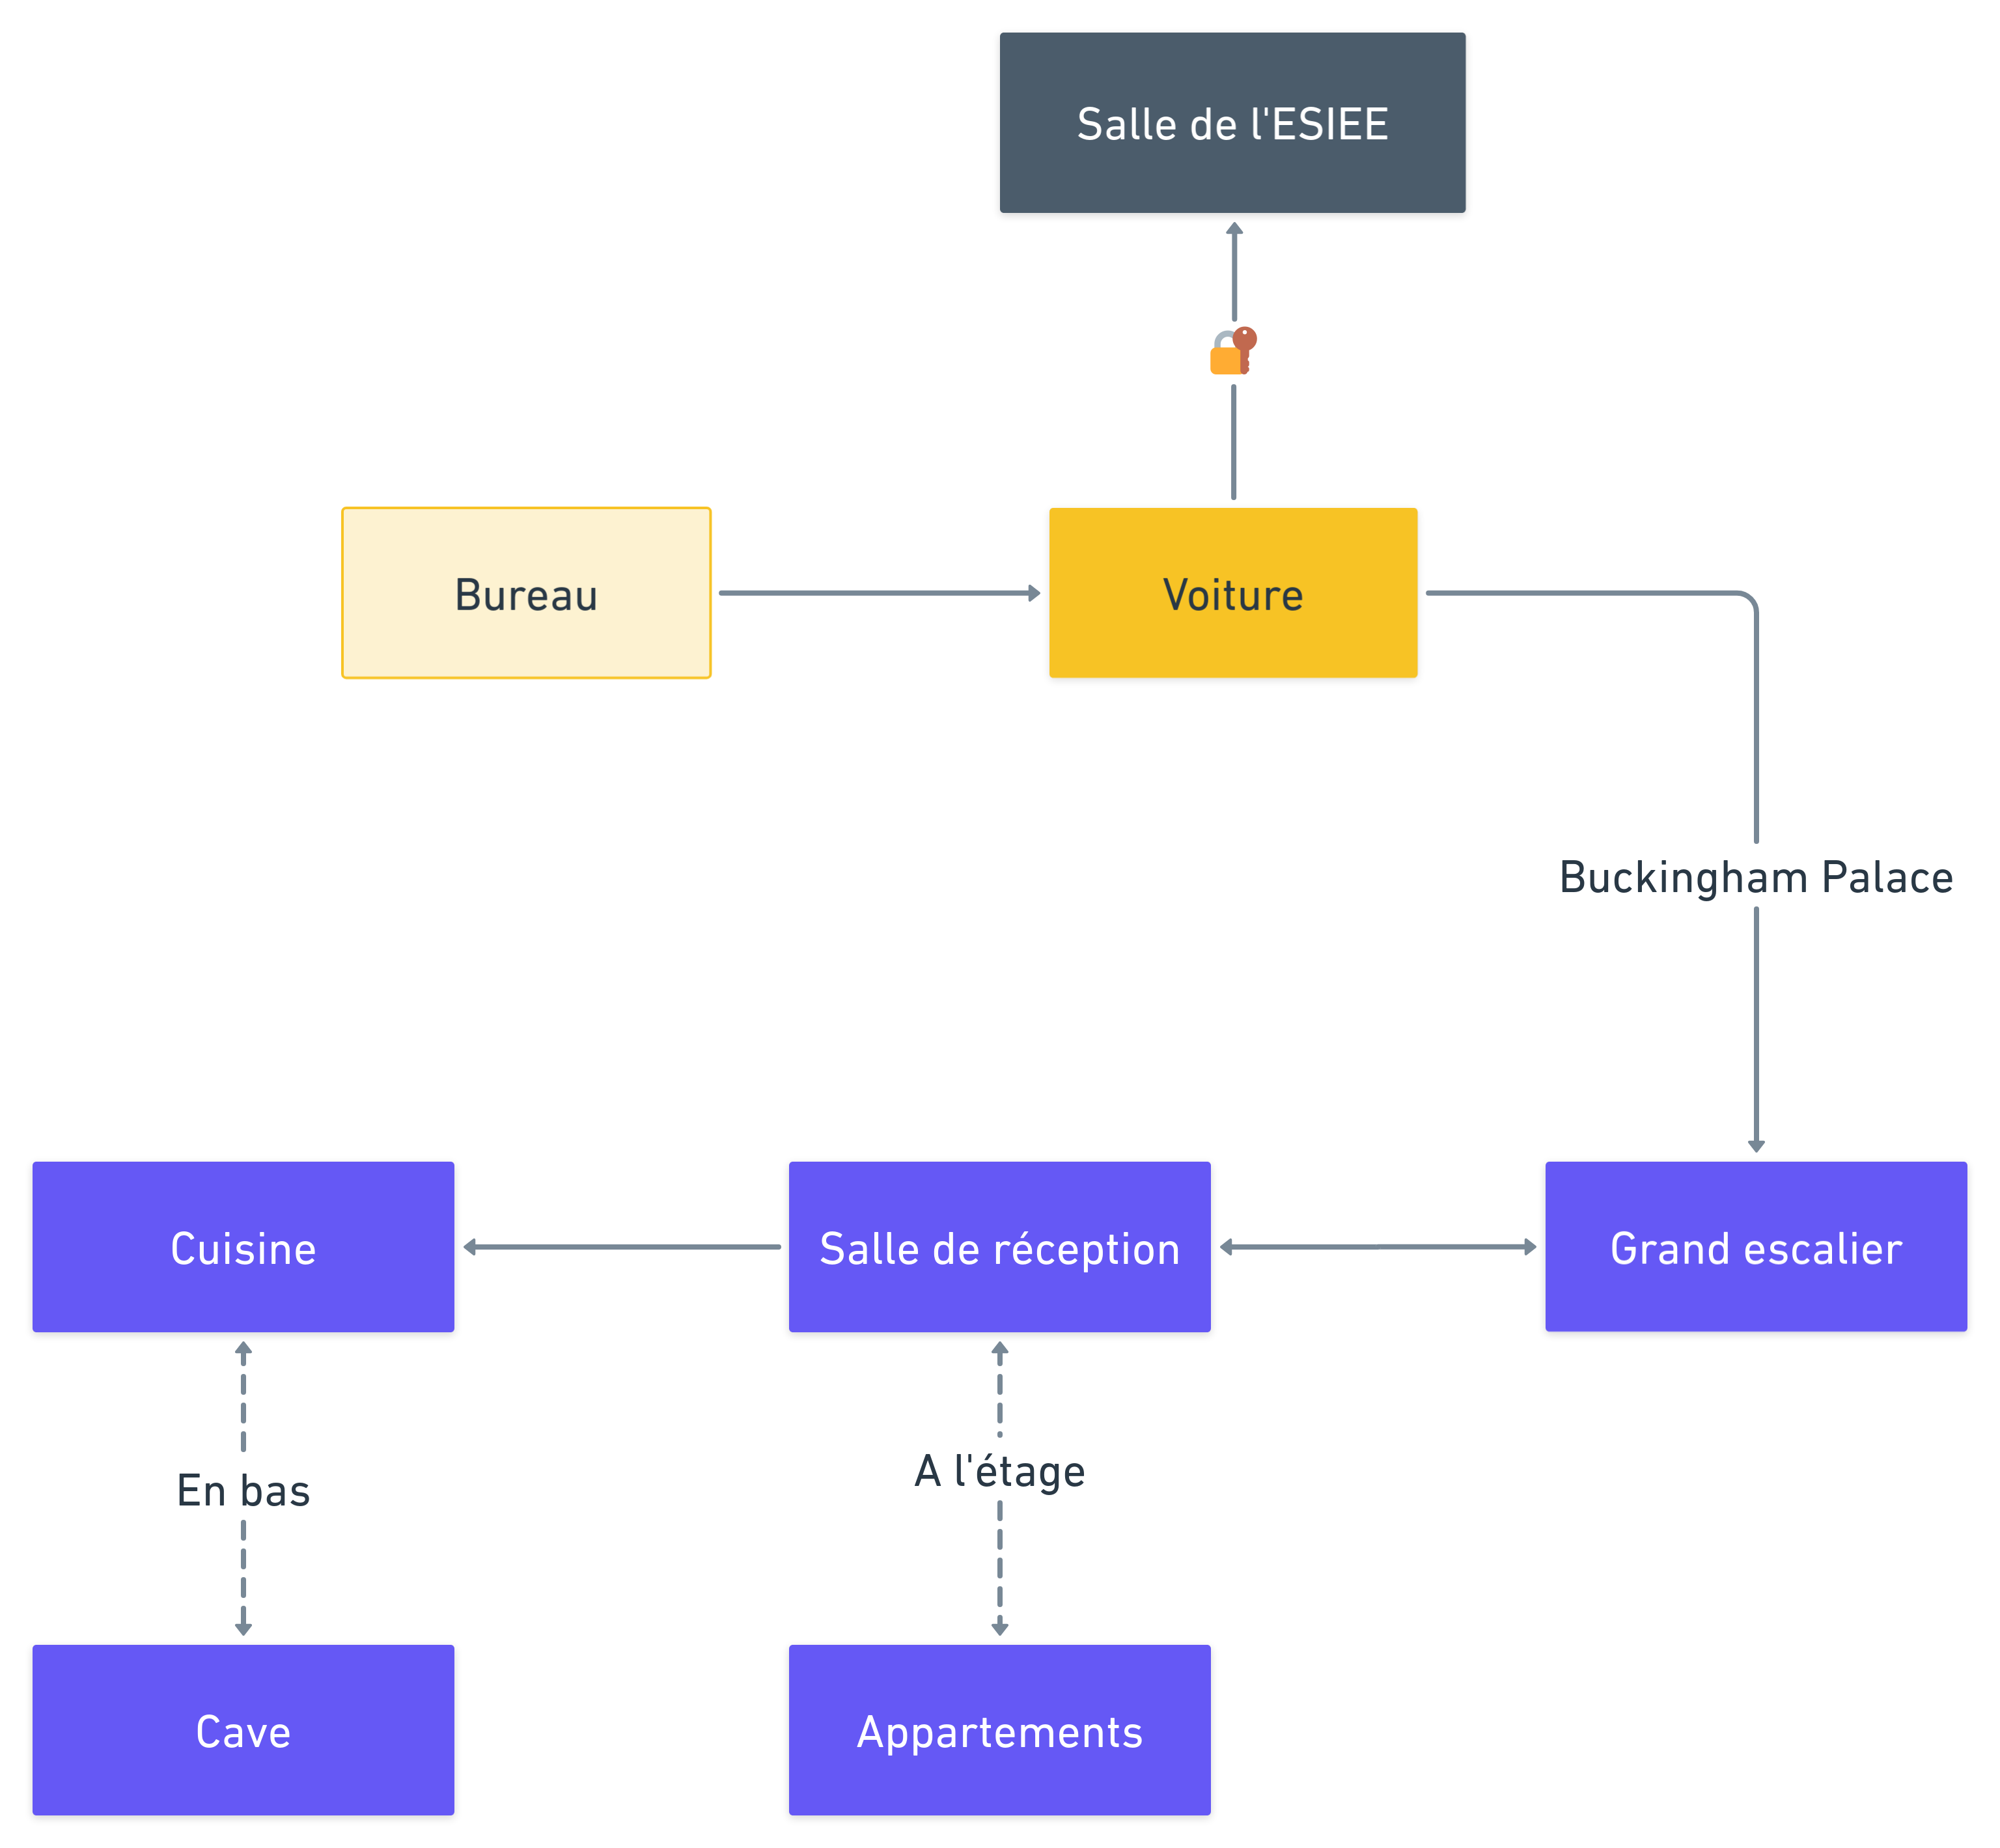
\includegraphics[width=\textwidth,height=\textheight,keepaspectratio]{./media/map.png}\\

\section{Détail des lieux, items, personnages}

\subsection{Lieux}

Seuls les lieux importants à l'avancement et à l'histoire du jeu sont listés ci-dessous.

\begin{description}[leftmargin=!,labelwidth=\widthof{\bfseries Bureau de Murphy}]
  \item [Bureau de Murphy] C'est le lieu où vous commencez votre aventure.
  \item [Voiture] La voiture vous permet de rejoindre certains lieux.
  \item [Grand escalier] C'est l'endroit où vous arrivez à Buckingham Palace.
  \item [Salle de réception] Là où la crise du corgi royal sera expliquée.
  \item [Salle de l'ESIEE] C'est dans cette salle de l'ESIEE que vous avez lancé ce jeu.
\end{description}

\subsection{Personnages}

De la même façon, cette liste ne comprend que les personnages essentiels au scénario. Certains personnages non-joueurs ne sont pas listés ici.

\begin{description}[leftmargin=!,labelwidth=\widthof{\bfseries Le Compilateur}]
  \item [Murphy Law] Le détective et aussi le personnage que vous incarnez. Son rôle est de mener l'enquête pour comprendre par quelles circonstances Le Joueur s'est retrouvé ici.
  \item [Le Narrateur] La voix que vous entendez quand vous jouez. Le Narrateur permet de décrire les scènes \& situations sans sortir de la narration. 
  \item [Le Joueur] C'est vous ! Cependant, Le Joueur est paradoxalement un personnage non jouable qui vous représente tout au long de  l'histoire dans le cadre de la méta-narration.
  \item [Le Compilateur] Le compilateur Java est le grand méchant de l'histoire. Son rôle, manipuler la structure du jeu pour que l'étudiant n'ait pas une note à la hauteur de son travail.
\end{description}

\section{Situations gagnantes et perdantes}

Le Joueur et Murphy Law seront confrontés à des situations de crises où des choix et décisions devront être prises, certains pourront entraîner la mort ou l'immobilisation des protagonistes et donc faire gagner Le Compilateur.\\
La liste des situations perdantes est la suivante :

\begin{description}[align=left,leftmargin=!,labelwidth=\widthof{\bfseries A Buckingham Palace}]
  \item [A Buckingham Palace] \begin{itemize}
    \item Vous ne retrouvez pas le corgi royal.
    \item Vous essayez de fouiller la Reine d'Angleterre.
  \end{itemize}
\end{description}

\section{Commentaires}

Murphy Law est une création originale de \href{http://scp-wiki.wikidot.com/murphy-law-hub}{la Fondation SCP}. Le personnage, les œuvres associées et ce jeu sont tous proposés sous licence \emph{Creative Commons Attribution-ShareAlike 3.0}
 
